\chapter{Marco teórico}

	Para realizar la estimación de la mirada de las personas en un plano virtual enfrente de ellas es necesario saber algunos conceptos, definiciones y algunos conocimientos que sirvan de apoyo al desarrollo del presente trabajo de tesis. En este capítulo se describen las bases para llevar a cabo el proyecto, dichas bases consisten principalmente de visión computacional, geometría proyectiva, algoritmos de aprendizaje supervisado, algoritmos de optimización numérica....

   %Añadir un parrafo de lo que aporta el de nosotros (plano)
   %Tomando en cuenta las consideraciones anteriores 
   %El proyecto de tesis propuesto además de estimar la pose de la cabeza mediante algoritmos de aprendizaje automático utilizará dichos algoritmos para asociarle a las cabezas humanas una región 

   
   \section{Detector de rostros de Viola y Jones}
  Como ya se ha mencionado anteriormente para estimar la mirada con precisión se necesita un sistema de detección y seguimiento de ojos además de múltiples cámaras y el sistema de estimación de pose de la cabeza, habiendo señalado lo anterior cabe destacar que el proyecto que se desarrollará más que estimar la mirada con precisión (además de la pose de la cabeza) representándola como un vector normal al iris,  se pretende estimar una región en un plano virtual enfrente de ellas, la región indicaría lo que están observando las personas de la escena que tienen enfrente. \\
   
   En el presente proyecto para la estimación de la pose de la cabeza de las personas en primer lugar se debe detectar dónde se encuentran los rostros (como se ha mencionado) para luego estimar su pose, ya que el sistema consiste de muchas etapas, se requiere que la detección se haga lo más rápido posible y eficientemente,  por lo tanto se decidió utilizar uno de los algoritmos de detección más utilizados y rápidos que existen: el clasificador basado en características tipo Haar en cascada. Este método fue propuesto por Paul Viola y Michael Jones en 2001 en el artículo Rapid Object Detection using a Boosted Cascade of Simple Features, el método consta principalmente de las siguientes etapas.
   
   \subsection{Imagen integral}
   En esta etapa se utiliza una representación intermedia de la imagen conocida como imagen integral o también conocida como tablas de áreas sumadas [Crow 1984]. En la imagen integral a cada pixel de la imagen se le asocia un valor representando la suma de los valores de los píxeles que se encuentran arriba y a la izquierda de él, así como también se le suma su valor de píxel. Este tipo de representación tiene como principal ventaja la rápida estimación del valor de los píxeles de subregiones de la imagen.
   \begin{figure}[htbp]
   	\centering
   	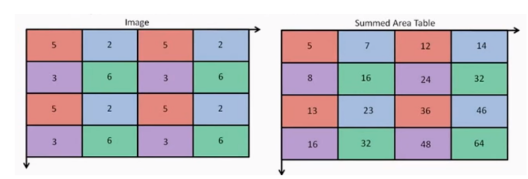
\includegraphics[width=0.7\textwidth]{./pictures/imagenIntegral}
   	\caption{Ejemplo de imagen integral}\label{fig: figura}
   \end{figure}
   El detector de Viola y Jones clasifica las imágenes basado en el valor de simples características, los sistemas basados en características operan muchos más rápido que los basados en píxeles. La imagen integral puede ser usada para estimar el valor de características tipo Haar, las características Haar se visualizan como rectángulos adyacentes blancos y negros, el valor que generan se calcula de la diferencia de la suma de los pixeles en el área blanca menos la suma de los del área negra, la adyacencia que presentan los rectángulos permite reutilizar algunos valores. El conjunto de características rectangulares ofrece una muy buena representación de imágenes la cual soporta un efectivo entrenamiento.
   
   \begin{figure}[htbp]
   	\centering
   	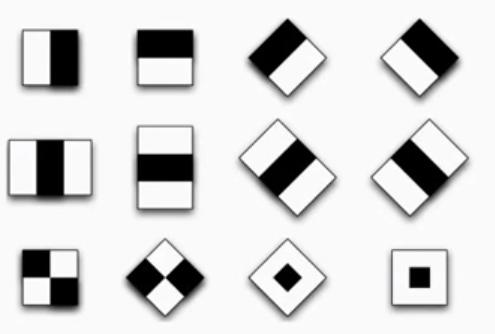
\includegraphics[width=0.4\textwidth]{./pictures/haar}
   	\caption{Características Haar}\label{fig: figura}
   \end{figure}
   
   \subsection{Algoritmo AdaBoost}
   Los métodos de Boosting [Friedman et al 2000] básicamente consisten en combinar la eficiencia de muchos clasificadores débiles para producir un poderoso consejo o comité clasificador. El algoritmo Adaboost es el método más usado y práctico de los algoritmos de Boosting. La idea general del AdaBoost consiste en que los ejemplos que son clasificados erróneamente obtienen mayor peso en las iteraciones siguientes, esto significa que los ejemplos que se encuentran cerca de la frontera de decisión son generalmente más difíciles de clasificar y por lo tanto se les asigna mayores pesos después de unas cuantas iteraciones. La idea de reasignación de pesos en el conjunto de entrenamiento es esencial en los métodos de Boosting.
   El detector de Viola y Jones se entrenó con conjuntos de imágenes etiquetadas como positivas y negativas, el algoritmo de AdaBoost fue utilizado para entrenar al clasificador y seleccionar un conjunto pequeño con las características Haar más importantes de una muy amplia biblioteca de posibles características. Como resultado final del proceso de entrenamiento el algoritmo de AdaBoost produce un clasificador robusto que tiene la forma de un perceptrón, una combinación de clasificadores débiles en el que cada clasificador tiene asociado una sola característica Haar y un umbral. Resumiendo lo anteriormente mencionado, la utilización del algoritmo de clasificación AdaBoost permite encontrar las características que mejor separan los ejemplos positivos de los negativos. Una de las ventajas clave por la cual fue elegido AdaBoost como algoritmo seleccionador de características por Viola y jones en su detector, es la increíble velocidad que presenta; usando AdaBoost, un clasificador de 200 características puede ser construido en alrededor 10-11 operaciones de procesador. Las primeras características seleccionadas por AdaBoost tienen mucho sentido y son fáciles de interpretar, una de esas característica parece enfocarse en la propiedad de que la región de los ojos es por lo regular más oscura que la región de la nariz y las mejillas.
   \begin{figure}[htbp]
   	\centering
   	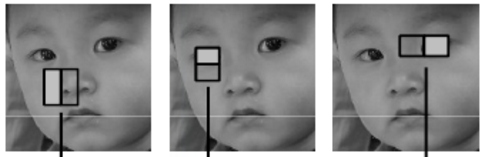
\includegraphics[width=0.7\textwidth]{./pictures/adaboost}
   	\caption{Características tipo Haar sobrepuestas}\label{fig: figura}
   \end{figure}
   
   \subsection{Filtro con estructura en cascada.}
   El último componente importante del Detector de Viola y Jones es la estructura en cascada que se forma con la combinación de unos cuantos clasificadores mejorados (boosted), estos clasificadores son usados para rechazar la mayor??a de las subregiones negativas (sin rostros de personas) y poner atención en regiones de la imagen más prometedoras, es decir, las regiones que presenten el rostro de alguna persona. Este método es muy eficiente ya que la mayor??a de las sub-ventanas o subregiones son rechazadas en etapas tempranas. Se le denominó estructura en ?cascada? debido a la forma que presenta al momento de procesar las sub- ventanas. Las sub-ventanas de la entrada del detector pasan a través de una serie de nodos, cada nodo toma una decisión binaria y dependiendo de la decisión la subregión se mueve al siguiente nodo o se rechaza. El número de clasificadores débiles presentes en cada nodo incrementa conforme la sub-ventana se va moviendo a los siguientes nodos, por ejemplo, en el primer nodo contiene un clasificador débil, el segundo 10, el tercero 25, el cuarto 50 y as?? sucesivamente. Teniendo pocos clasificadores en etapas tempranas es otra forma de mejorar la velocidad del detector y esto de alguna forma compensa el costo de evaluar cada caracter??stica Haar en diferentes escalas y posiciones de la imagen.
   \begin{figure}[htbp]
   	\centering
   	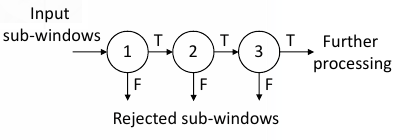
\includegraphics[width=0.7\textwidth]{./pictures/cascada}
   	\caption{Diagrama de nodos}\label{fig: figura}
   \end{figure}
   
   El detector de rostros descrito en esta sección tiene incontables aplicaciones y debido la velocidad de la detección puede ser utilizado en aplicaciones que requieran detección en tiempo real. Uno de los aspectos más interesantes del método de Viola y Jones es que no se limita a la detección de rostros, puede ser modificado para sistemas detectores de otro tipo de patrones en las imágenes, por ejemplo automóviles, peatones y recientemente utilizado para la detección de la enfermedad de Chagas, mediante las muestras de sangre de los infectados [Uc Cetina et al 2015].
   \begin{figure}[htbp]
   	\centering
   	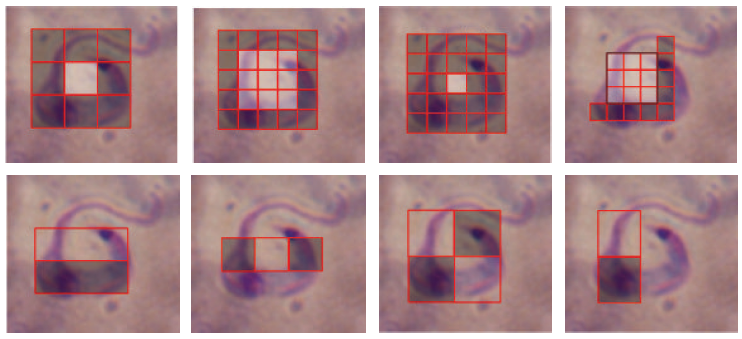
\includegraphics[width=0.7\textwidth]{./pictures/chagas}
   	\caption{Detección de chagas en la sangre mediante el método de Viola y Jones}\label{fig: figura}
   \end{figure}
   
   \section{Matrices de Rotación}
   \section{Homografía}
   \section{Modelo pinhole de cámara}
   \section{Calibración de cámaras y corrección de imágenes}
   \section{Optimización numérica y Levenberg-Marquardt}
   \section{Aprendizaje Automático}
   \section{Redes neuronales artificiales}

